\section{Our Approach}
\label{approach}


\begin{figure*}[ht]
\centering
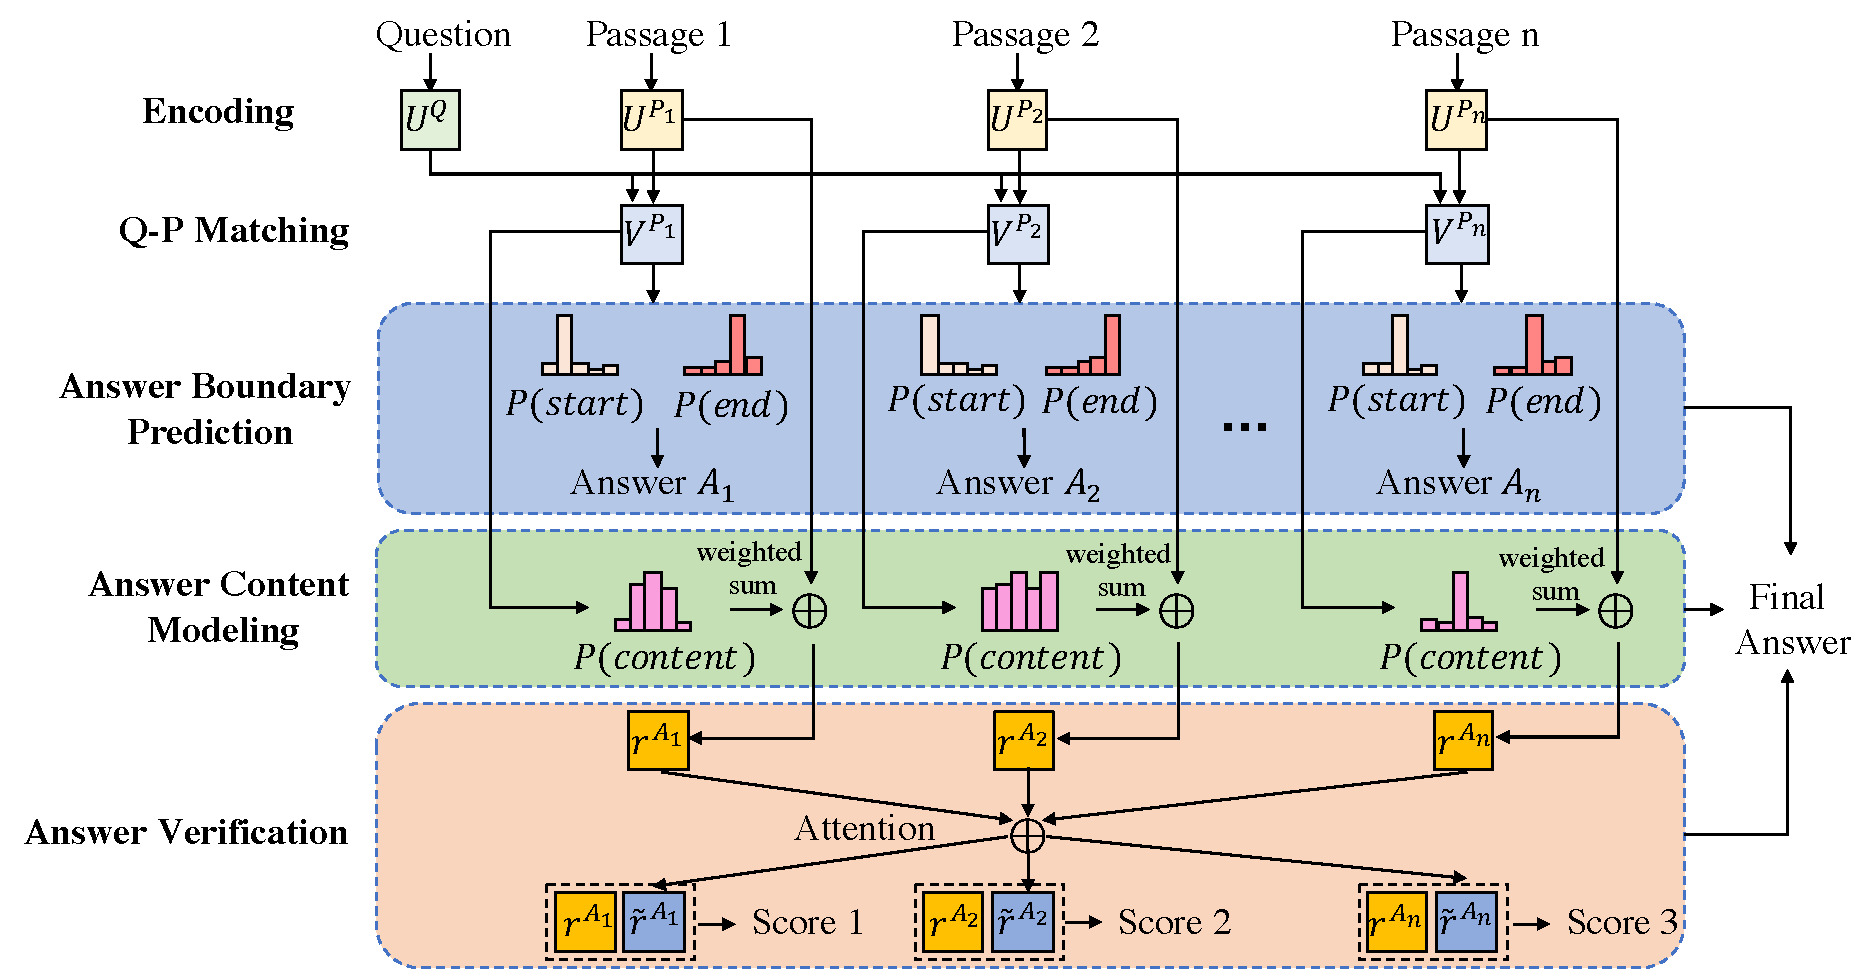
\includegraphics[width=\textwidth]{architecture.pdf}

\caption{Overview of our method for multi-passage machine reading comprehension}
\label{fig:architecture}
\end{figure*}

\figref{fig:architecture} gives an overview of our multi-passage MRC model
which is mainly composed of three modules including answer boundary prediction, answer content modeling and answer verification.
First of all, we need to model the question and passages. Following \newcite{bidaf}, we compute the question-aware representation for each passage (\secref{modeling}).
Based on this representation, we employ a Pointer Network \cite{pointer-net} to predict the start and end position of the answer in the module of answer boundary prediction (\secref{boundary}). 
At the same time, with the answer content model (\secref{content}), we estimate whether each word should be included in the answer and thus obtain the answer representations. 
Next, in the answer verification module (\secref{verification}), each answer candidate can attend to the other answer candidates to collect supportive information and we compute one score for each candidate to indicate whether it is correct or not according to the verification. 
The final answer is determined by not only the boundary but also the answer content and its verification score (\secref{train}).

%\figref{fig:architecture} gives an overview of our multi-passage reading comprehension model. First, we encode the question and passages separately using LSTM \cite{lstm} and then we follow \newcite{bidaf} to couple the query and context vectors. Based on the query-aware representation of the passages, we employ a Pointer Network \cite{pointer-net} to predict the start and end position of the answer. Beyond that, with the content model (\secref{content}), we compute whether each word should be included in the content of the answer and thus obtain a representation of the answer. Next, The answer verification (\secref{verification}) is conducted among the answers from different passages. Each answer can attend to the other answers to collect supportive information and then one score is computed for each answer to indicate whether this answer is correct or not after verification. The final answer is determined by not only the boundary but also the answer content and its verification score. 

%\subsection{Reading Comprehension Model}
\subsection{Question and Passage Modeling}
\label{modeling}
%\label{rc}
%First, we formally present the details of passage modeling process.
%Given a question $\matr{Q}$ and a set of passages 
%$\{\matr{P}_i\}$  retrieved by search engines, 
%our task is to find the best concise answer that could answer the question. 
%Then, we need to model the passages with consideration of the question.

Given a question $\matr{Q}$ and a set of passages 
$\{\matr{P}_i\}$  retrieved by search engines, 
our task is to find the best concise answer to the question. First, we formally present the details of modeling the question and passages.
%We first follow previous methods \cite{bidaf, match-lstm} to conduct the classic reading comprehension, while the difference here is that we will predict one answer candidate for each passage. 

\paragraph{Encoding} We first map each word into the vector space by concatenating its word embedding and sum of its character embeddings. Then we employ bi-directional LSTMs (BiLSTM) to encode the question $\matr{Q}$ and passages $\{\matr{P}_i\}$ as follows:
%\begin{small}
\begin{align}
%	U^Q &= [ \overrightarrow{\textrm{LSTM}}(Q), \overleftarrow{\textrm{LSTM}}(Q) ] \\
%	U^{P_i} &= [ \overrightarrow{\textrm{LSTM}}(P_i), \overleftarrow{\textrm{LSTM}}(P_i) ] 
%U^Q &= \textrm{BiLSTM}_Q(Q) \\  
%U^{P_i} &= \textrm{BiLSTM}_P(P_i)
{\vec{u}}_t^Q & = \textrm{BiLSTM}_Q({\vec{u}}_{t-1}^Q, [{\vec{e}}_t^Q, {\vec{c}}_t^Q]) \\
{\vec{u}}_t^{P_i} & = \textrm{BiLSTM}_P({\vec{u}}_{t-1}^{P_i}, [{\vec{e}}_t^{P_i}, {\vec{c}}_t^{P_i}])
\end{align}
%\end{small}
%The resulting matrices $U^Q \in \mathbb{R}^{2d
%\times |Q|}$ and $U^{P_i} \in \mathbb{R}^{2d
%\times |P_i|}$ are the hidden vectors of all the words in the question and passage. 
\noindent where ${\vec{e}}_t^Q$, ${\vec{c}}_t^Q$, ${\vec{e}}_t^{P_i}$, ${\vec{c}}_t^{P_i}$ are the word-level and character-level embeddings of the $t^{th}$ word. ${\vec{u}}_t^Q$ and ${\vec{u}}_t^{P_i}$ are the encoding vectors of the $t^{th}$ words in $\matr{Q}$ and $\matr{P}_i$ respectively.
Unlike previous work \cite{rnet} that simply concatenates all the passages, we process the passages independently at the encoding and matching steps. 

\paragraph{Q-P Matching} One essential step in MRC is to match the question with passages so that important information can be highlighted. We use the Attention Flow Layer \cite{bidaf} to conduct the Q-P matching in two directions. The similarity matrix $\matr{S} \in \mathbb{R}^{|\matr{Q}|
\times |\matr{P}_i|}$ between the question and passage $i$ is changed to a simpler version, where the similarity between the $t^{th}$ word in the question and the $k^{th}$ word in passage $i$ is computed as:
%\begin{small}
\begin{equation}
	\matr{S}_{t,k} = {{\vec{u}}_t^Q}^{\intercal} \cdot {\vec{u}}_k^{P_i}
\end{equation}
%\end{small}
%where ${\vec{u}_t^Q}^{\intercal}$ is the inversion of ${\vec{u}}_t^Q$
%\begin{equation}
%	S = {U^Q}^{\intercal} U^{P_i}
%\end{equation} 

Then the context-to-question attention and question-to-context attention is applied strictly following \newcite{bidaf} to obtain the question-aware passage representation $\{{\vec{\tilde{u}}}_t^{P_i}\}$.
%$M^{P_i} \in \mathbb{R}^{8d\times |P_i|}$. 
We do not give the details here due to space limitation. Next, another BiLSTM is applied in order to fuse the contextual information and get the new representation for each word in the passage, which is regarded as the match output:
%\begin{small}
\begin{equation}
	{\vec{v}}_t^{P_i} = \textrm{BiLSTM}_M({\vec{v}}_{t-1}^{P_i}, {\vec{\tilde{u}}}_t^{P_i})
\end{equation}
%\end{small}
%\begin{align}
%V^{P_i} &= \textrm{BiLSTM}_M(M^{P_i}) 
%\end{align}

%where $V^{P_i} \in \mathbb{R}^{2d
%\times |P_i|}$ is the new representation of all the words in the passage after matching.
Based on the passage representations, we introduce the three main modules of our model.

\subsection{Answer Boundary Prediction}
\label{boundary}
%\paragraph{Answer Boundary Prediction} 
%We first follow previous methods \cite{bidaf, match-lstm} to conduct the classic reading comprehension, while the difference here is that we will predict one answer candidate for each passage.

To extract the answer span from passages, mainstream studies try to locate the boundary of the answer, which is called boundary model. Following \cite{match-lstm}, we employ Pointer Network \cite{pointer-net} to compute the probability of each word to be the start or end position of the span:
%\begin{small}
\begin{align}
	g_k^t &= {\vec{w}_{1}^{a}}^{\intercal} \tanh ( \matr{W}_{2}^a [\vec{v}_k^{P}, \vec{h}_{t-1}^{a}] ) \\
	{\alpha}_k^t &= \textrm{exp} (g_k^t) / \sum\nolimits_{j=1}^{|\matr{P}|} \textrm{exp} (g_j^t) \\
	\vec{c}_t &= \sum\nolimits_{k=1}^{|\matr{P}|} {\alpha}_k^t \vec{v}_k^{P} \\
	\vec{h}_t^a &= \textrm{LSTM} (\vec{h}_{t-1}^a, \vec{c}_t)
\end{align}
%\end{small}

%Since the probability are also used to compare answers from different passages, we concat the representation of all passages $\{V^{P_i}\}$ to be $V^P \in \mathbb{R}^{2d
%\times |P|}$ so that the probabilities are comparable across passage after the softmax layer. Then the boundary pointer can be formulated as follows:
%
%\begin{align}
%\small
%F_k &= \tanh(W_v V^P \notag \\
%	&\phantom{{}=1}\phantom{{}=1}+ (W_a h_{k-1}^a + b_a) \otimes e_{(P)}) \\
%{p}_{k} &= \textrm{softmax}(v_a^\intercal F_k + c_a 
%\otimes e_{(P)}) \\
%h_k^a &= \textrm{LSTM}_{A}(V^P {p}_{k}^{\intercal}, h_{k-1}^a )
%\end{align}

By utilizing the attention weights, the probability of the $k^{th}$ word in the passage to be the start and end position of the answer is obtained as ${\alpha}_k^1$ and ${\alpha}_k^2$. It should be noted that the pointer network is applied to the concatenation of all passages, which is denoted as $\textrm{P}$ so that the probabilities are comparable across passages. This boundary model can be trained by minimizing the negative log probabilities of the true start and end indices:
%\begin{small}
\begin{equation}
	\mathcal{L}_{boundary} = - \frac{1}{N} \sum_{i=1}^N (\log {\alpha}_{y_i^{1}}^1 + \log {\alpha}_{y_i^{2}}^2)
\end{equation}
%\end{small}
\noindent where $N$ is the number of samples in the dataset and $y_i^{1}$, $y_i^{2}$ are the gold start and end positions.

%After that, for each passage, we extract the text span that has the maximum boundary score, which is computed as the product of its start probability and end probability. We denote the answer candidate from passage $i$ as $A^i$ and the corresponding boundary score as $\textrm{Score}_{boundary}(A^i)$
%$s_{b}^{A^i}$.

\subsection{Answer Content Modeling}
\label{content}

%Even though the boundary model shows its effectiveness in extracting the answer span, we find that only us

%Now we have extracted the answer candidate from each passage. However, before we conduct the answer verification, it is still a problem that how can we model the meaning of those answers. An intuitive method is to compute the representation based on the extracted answer. However, this will divide the whole model into two parts that cannot be trained end-to-end. Therefore, we propose a novel method that can obtain the representation based on probability. 

Previous work employs the boundary model to find the text span with the maximum boundary score as the final answer. However, in our context, besides locating the answer candidates, we also need to model their meanings in order to conduct the verification. 
An intuitive method is to compute the representation of the answer candidates separately after extracting them, 
but it could be hard to train such model end-to-end.
Here, we propose a novel method that can obtain the representation of the answer candidates based on probabilities. 
%An intuitive method is to compute the representation based on the extracted answer. However, this will divide the whole model into two parts that cannot be trained end-to-end. Therefore, we propose a novel method that can obtain the representation of the answer based on probabilities. 

Specifically, we change the output layer of the classic MRC model. Besides predicting the boundary probabilities for the words in the passages, we also predict whether each word should be included in the content of the answer. The content probability of the $k^{th}$ word is computed as:
%\begin{small}
\begin{align}
	p_k^c &= \textrm{sigmoid} ({\vec{w}_{1}^{c}}^{\intercal} \textrm{ReLU} (\matr{W}_{2}^c \vec{v}_k^{P_i}) )
%	a_k^c &= \textrm{exp} (s_k^c) / \sum\nolimits_{j=1}^{|\matr{P}^i|} \textrm{exp} (s_j^c)
\end{align}
%\end{small}

Training this content model is also quite intuitive. We transform the boundary labels into a continuous segment, which means the words within the answer span will be labeled as 1 and other words will be labeled as 0. In this way, we define the loss function as the averaged cross entropy:
%\begin{small}
\begin{equation}
\begin{split}
	\mathcal{L}_{content} = & - \frac{1}{N} \frac{1}{|\textrm{P}|} \sum_{i=1}^N \sum_{j=1}^{|P|} [  y_k^c\log p_{k}^c \\ 
	& + (1-y_k^c)\log (1 - p_{k}^c)]
\end{split}
\end{equation}
%\end{small}

The content probabilities provide another view to measure the quality of the answer in addition to the boundary. Moreover, with these probabilities, we can represent the answer from passage $i$ as a weighted sum of all the word embeddings in this passage:
%\begin{small}
\begin{align}
	\vec{r}^{A_i} = \frac{1}{|\matr{P}_{i}|}\sum\nolimits_{k=1}^{|\matr{P}_{i}|} p_k^c [{\vec{e}}_k^{P_i}, {\vec{c}}_k^{P_i}]
\end{align}
%\end{small}

\subsection{Cross-Passage Answer Verification}
\label{verification}

The boundary model and the content model focus on extracting and modeling the answer within a single passage respectively, 
with little consideration of the cross-passage information. 
% The boundary and content model focus on extracting and modeling the answer within a single passage with little consideration of cross-passage information. 
However, as is discussed in \secref{introduction}, there could be multiple answer candidates from different passages
%the answer candidates from different passages are usually quite different 
and some of them may mislead the MRC model to make an incorrect prediction. It's necessary to aggregate the information from different passages and choose the best one from those candidates. Therefore, we propose a method to enable the answer candidates to exchange information and verify each other through the cross-passage answer verification process. 

Given the representation of the answer candidates from all passages $\{\vec{r}^{A_{i}}\}$, each answer candidate then attends to other candidates to collect supportive information via attention mechanism:
%\begin{small}
\begin{align}
	s_{i, j} &= 
	 \begin{cases}
 		0, & \text{if } i=j, \\
 		{\vec{r}^{A_i}}^{\intercal} \cdot \vec{r}^{A_j},  & \text{otherwise}	
 \end{cases}
 \\
	{\alpha}_{i, j} &= \textrm{exp} (s_{i, j}) / \sum\nolimits_{k=1}^{n} \textrm{exp} (s_{i, k}) \\
	\vec{\tilde{r}}^{A_i} &= \sum\nolimits_{j=1}^{n} {\alpha}_{i, j}\vec{r}^{A_j}
\end{align}
%\end{small}

Here $\vec{\tilde{r}}^{A_{i}}$ is the collected verification information from other passages based on the attention weights. Then we pass it together with the original representation $\vec{r}^{A_{i}}$ to a fully connected layer:
%\begin{small}
\begin{align}
	g_{i}^v &= {\vec{w}^v}^{\intercal} [\vec{r}^{A_i}, \vec{\tilde{r}}^{A_i}, \vec{r}^{A_i} \odot \vec{\tilde{r}}^{A_i} ]
\end{align}
%\end{small}
We further normalize these scores over all passages to get the verification score for answer candidate $A_i$:
%\begin{small}
\begin{equation}
%	p_i^v = g_i^v / \sum\nolimits_{j=1}^{n} g_j^v
	p_i^v = \textrm{exp} (g_i^v) / \sum\nolimits_{j=1}^{n} \textrm{exp} (g_j^v)
\end{equation}
%\end{small}

In order to train this verification model, we take the answer from the gold passage as the gold answer. And the loss function can be formulated as the negative log probability of the correct answer:
%\begin{small}
\begin{equation}
	\mathcal{L}_{verify} = - \frac{1}{N} \sum_{i=1}^N \log p_{y_i^v}^{v}
\end{equation}
%\end{small}
where $y_i^v$ is the index of the correct answer in all the answer candidates of the $i^{th}$ instance . 

\subsection{Joint Training and Prediction}
\label{train}

As is described above, we define three objectives for the reading comprehension model over multiple passages: 1. finding the boundary of the answer; 2. predicting whether each word should be included in the content; 3. selecting the best answer via cross-passage answer verification. According to our design, these three tasks can share the same embedding, encoding and matching layers. Therefore, we propose to train them together as multi-task learning \cite{multi-task}. The joint objective function is formulated as follows:
%\begin{small}
\begin{equation}
	\mathcal{L} = \mathcal{L}_{boundary} + \beta_{1} \mathcal{L}_{content} + \beta_{2} \mathcal{L}_{verify}
\end{equation}
%\end{small}
where $\beta_1$ and $\beta_2$ are two hyper-parameters that control the weights of those tasks.

When predicting the final answer, we take the boundary score, content score and verification score into consideration. 
We first extract the answer candidate $A_i$ that has the maximum boundary score from each passage $i$. This boundary score is computed as the product of the start and end probability of the answer span. Then for each answer candidate $A_i$, we average the content probabilities of all its words as the content score of $A_i$. And we can also predict the verification score for $A_i$ using the verification model. Therefore, the final answer can be selected from all the answer candidates according to the product of these three scores. 
 